\documentclass[10pt,a4paper]{article}
\usepackage[margin=2.2cm]{geometry}
\usepackage{amsmath,amssymb}
\usepackage{booktabs,tabularx,array}
\usepackage{graphicx}
\usepackage[table]{xcolor}
\usepackage{enumitem}
\usepackage{algorithm}
\usepackage{algpseudocode}
\usepackage[hidelinks]{hyperref}
\usepackage{microtype}
\usepackage{float}
\setlist{itemsep=2pt,topsep=3pt}
\renewcommand{\arraystretch}{1.15}
\newcolumntype{L}{>{\raggedright\arraybackslash}X}
\newcommand{\fiftypaperSaWOneRule}{100\%}
\newcommand{\fiftypaperSaExRule}{92\%}
\newcommand{\fiftypaperSaWOneSa}{100\%}
\newcommand{\fiftypaperSaGap}{+0.0\%}
\newcommand{\fiftypaperSaBetter}{0/12}
\newcommand{\fiftypaperSaAtRule}{+0.0\%}
\newcommand{\fiftypaperSaAm}{4.50}
\newcommand{\fiftypaperSaCens}{0\%}
\newcommand{\fiftypaperClWOneRule}{100\%}
\newcommand{\fiftypaperClExRule}{50\%}
\newcommand{\fiftypaperClWOneSa}{100\%}
\newcommand{\fiftypaperClGap}{+26.9\%}
\newcommand{\fiftypaperClBetter}{1/12}
\newcommand{\fiftypaperClAtRule}{+35.1\%}
\newcommand{\fiftypaperClAm}{4.08}
\newcommand{\fiftypaperClCens}{0\%}
\newcommand{\fiftypaperLiuWOneRule}{100\%}
\newcommand{\fiftypaperLiuExRule}{75\%}
\newcommand{\fiftypaperLiuWOneSa}{100\%}
\newcommand{\fiftypaperLiuGap}{+2.0\%}
\newcommand{\fiftypaperLiuBetter}{4/12}
\newcommand{\fiftypaperLiuAtRule}{+2.0\%}
\newcommand{\fiftypaperLiuAm}{4.33}
\newcommand{\fiftypaperLiuCens}{0\%}
\newcommand{\fiftyringSaWOneRule}{100\%}
\newcommand{\fiftyringSaExRule}{67\%}
\newcommand{\fiftyringSaWOneSa}{100\%}
\newcommand{\fiftyringSaGap}{+0.0\%}
\newcommand{\fiftyringSaBetter}{0/12}
\newcommand{\fiftyringSaAtRule}{+0.0\%}
\newcommand{\fiftyringSaAm}{3.33}
\newcommand{\fiftyringSaCens}{0\%}
\newcommand{\fiftyringClWOneRule}{100\%}
\newcommand{\fiftyringClExRule}{33\%}
\newcommand{\fiftyringClWOneSa}{100\%}
\newcommand{\fiftyringClGap}{+2.9\%}
\newcommand{\fiftyringClBetter}{5/12}
\newcommand{\fiftyringClAtRule}{+16.8\%}
\newcommand{\fiftyringClAm}{2.83}
\newcommand{\fiftyringClCens}{0\%}
\newcommand{\fiftyringLiuWOneRule}{100\%}
\newcommand{\fiftyringLiuExRule}{67\%}
\newcommand{\fiftyringLiuWOneSa}{92\%}
\newcommand{\fiftyringLiuGap}{$-$0.6\%}
\newcommand{\fiftyringLiuBetter}{6/12}
\newcommand{\fiftyringLiuAtRule}{$-$0.9\%}
\newcommand{\fiftyringLiuAm}{3.00}
\newcommand{\fiftyringLiuCens}{0\%}
\newcommand{\fiftycoreSaWOneRule}{83\%}
\newcommand{\fiftycoreSaExRule}{50\%}
\newcommand{\fiftycoreSaWOneSa}{100\%}
\newcommand{\fiftycoreSaGap}{+0.0\%}
\newcommand{\fiftycoreSaBetter}{0/12}
\newcommand{\fiftycoreSaAtRule}{+0.0\%}
\newcommand{\fiftycoreSaAm}{6.83}
\newcommand{\fiftycoreSaCens}{0\%}
\newcommand{\fiftycoreClWOneRule}{100\%}
\newcommand{\fiftycoreClExRule}{67\%}
\newcommand{\fiftycoreClWOneSa}{100\%}
\newcommand{\fiftycoreClGap}{$-$38.2\%}
\newcommand{\fiftycoreClBetter}{12/12}
\newcommand{\fiftycoreClAtRule}{$-$39.5\%}
\newcommand{\fiftycoreClAm}{5.00}
\newcommand{\fiftycoreClCens}{0\%}
\newcommand{\fiftycoreLiuWOneRule}{100\%}
\newcommand{\fiftycoreLiuExRule}{67\%}
\newcommand{\fiftycoreLiuWOneSa}{83\%}
\newcommand{\fiftycoreLiuGap}{$-$40.2\%}
\newcommand{\fiftycoreLiuBetter}{12/12}
\newcommand{\fiftycoreLiuAtRule}{$-$42.1\%}
\newcommand{\fiftycoreLiuAm}{5.00}
\newcommand{\fiftycoreLiuCens}{0\%}
\newcommand{\fiftyLiuBetterAll}{22/36}
\newcommand{\fiftyLiuWOneRuleAll}{36/36}
\newcommand{\fiftyTailLo}{0.96}\newcommand{\fiftyTailHi}{1.00}
\newcommand{\fiftypaperLiuKtwo}{0.79}
\newcommand{\fiftyringLiuKtwo}{0.82}
\newcommand{\fiftycoreLiuKtwo}{0.52}
\newcommand{\fortypaperSaWOneRule}{100\%}
\newcommand{\fortypaperSaExRule}{75\%}
\newcommand{\fortypaperSaWOneSa}{100\%}
\newcommand{\fortypaperSaGap}{+0.0\%}
\newcommand{\fortypaperSaBetter}{0/12}
\newcommand{\fortypaperSaAtRule}{+0.0\%}
\newcommand{\fortypaperSaAm}{4.83}
\newcommand{\fortypaperSaCens}{0\%}
\newcommand{\fortypaperClWOneRule}{92\%}
\newcommand{\fortypaperClExRule}{50\%}
\newcommand{\fortypaperClWOneSa}{92\%}
\newcommand{\fortypaperClGap}{+6.1\%}
\newcommand{\fortypaperClBetter}{2/12}
\newcommand{\fortypaperClAtRule}{+25.6\%}
\newcommand{\fortypaperClAm}{4.33}
\newcommand{\fortypaperClCens}{0\%}
\newcommand{\fortypaperLiuWOneRule}{100\%}
\newcommand{\fortypaperLiuExRule}{50\%}
\newcommand{\fortypaperLiuWOneSa}{100\%}
\newcommand{\fortypaperLiuGap}{$-$5.5\%}
\newcommand{\fortypaperLiuBetter}{9/12}
\newcommand{\fortypaperLiuAtRule}{$-$2.7\%}
\newcommand{\fortypaperLiuAm}{4.25}
\newcommand{\fortypaperLiuCens}{0\%}
\newcommand{\fortyringSaWOneRule}{100\%}
\newcommand{\fortyringSaExRule}{50\%}
\newcommand{\fortyringSaWOneSa}{100\%}
\newcommand{\fortyringSaGap}{+0.0\%}
\newcommand{\fortyringSaBetter}{0/12}
\newcommand{\fortyringSaAtRule}{+0.0\%}
\newcommand{\fortyringSaAm}{3.50}
\newcommand{\fortyringSaCens}{0\%}
\newcommand{\fortyringClWOneRule}{100\%}
\newcommand{\fortyringClExRule}{33\%}
\newcommand{\fortyringClWOneSa}{75\%}
\newcommand{\fortyringClGap}{+3.7\%}
\newcommand{\fortyringClBetter}{3/12}
\newcommand{\fortyringClAtRule}{+17.0\%}
\newcommand{\fortyringClAm}{3.00}
\newcommand{\fortyringClCens}{0\%}
\newcommand{\fortyringLiuWOneRule}{100\%}
\newcommand{\fortyringLiuExRule}{67\%}
\newcommand{\fortyringLiuWOneSa}{100\%}
\newcommand{\fortyringLiuGap}{$-$2.9\%}
\newcommand{\fortyringLiuBetter}{10/12}
\newcommand{\fortyringLiuAtRule}{$-$4.6\%}
\newcommand{\fortyringLiuAm}{3.17}
\newcommand{\fortyringLiuCens}{0\%}
\newcommand{\fortyLiuBetterAll}{19/24}
\newcommand{\fortyLiuWOneRuleAll}{24/24}
\newcommand{\fortypaperLiuKtwo}{0.66}
\newcommand{\fortyringLiuKtwo}{0.77}

\makeatletter\newcommand\inputtab[1]{\@@input #1 }\makeatother % \input inside tabular breaks \midrule

\title{Implementing Liu \emph{et al.}\ (IEEE IoT-J 2022) as a Baseline\\for the Fleet-Sizing Rule:
Required Changes, Procedure and Results}
\author{Implementation report}
\date{\today}

\begin{document}
\maketitle

\begin{abstract}
\noindent
We re-implemented the multi-population genetic algorithm (MPGA) of Liu, Guo, Li and Song,
``AoI-Minimal Task Assignment and Trajectory Optimization in Multi-UAV-Assisted IoT Networks'' (IEEE
IoT-J, 2022), as an external baseline for the fleet-sizing paper. We adapted it to that paper's system
model: one shared energy inventory split over $K$ UAVs, nonstop sortie operation from a central depot,
and priority-weighted age at collection. This report lists every change needed and why, the exact steps
followed, the tests, and the results on the three layout families (clustered ``paper'', ring, core) at
$M=50$ sensors and $E_{\max}=1.5$\,MJ. We compare against our simulated-annealing (SA) planner, with
the published cluster patrol as a reference. Across the three families, the adapted Liu planner's
optimal fleet size lies within one UAV of the closed-form point predictor $\ell$ in
\fiftyLiuWOneRuleAll{} instances, and its time-average AoI at its own optimum is lower than SA's in
\fiftyLiuBetterAll{} instances.
\end{abstract}

%=====================================================================================================
\section{The two methods being compared}

\paragraph{Our planner (the original).}
$K$ UAVs share a usable energy inventory $U=(1-\rho)E_{\max}$, so each sortie has a budget of $U/K$.
Every time a UAV lands it immediately relaunches and plans one sortie. The planner solves a
set-orienteering problem: maximise $\sum_j w_j\hat a_j$ over sensors not already committed to another
UAV (depot-mediated exclusion), subject to the sortie budget. It uses simulated annealing with 1{,}200
iterations, a cost-aware eject-and-insert repair move, and a greedy seed. The fleet-sizing rule gives the
point predictor $\ell=\min(\lfloor K_{\mathrm{reach}}\rfloor,\operatorname{round}K_{\mathrm{commute}})$.

\paragraph{Liu \emph{et al.}\ (the baseline).}
UAVs leave a data center, collect from their assigned sensors in order, meet at an interaction point
(IPT) to share data, deliver it to users, and return. The objective is the average AoI of the data the
users receive, subject to a per-UAV energy limit and a minimum separation between UAVs. The joint
assignment-and-routing subproblem is solved by an MPGA. A chromosome is one permutation of all sensors
(followed by all users), cut into one segment per UAV by breakpoints. The GA runs $N_p=8$ populations of
$N_0=60$ individuals for $N_{\mathrm{iter}}=100$ generations. It uses roulette selection on a normalised
fitness, with the population's or the global best sometimes chosen as a parent; order (sequential)
crossover; swap, inversion and slide mutations; and a breakpoint-update operator that balances route
lengths. Each population has its own $p_{cr}\sim\mathcal U[0.5,0.95]$ and $p_{mu}\sim\mathcal U[0.05,0.3]$.
The paper also gives an improved global K-means + dynamic-programming hybrid, and a Fermat--Weber
step that places the IPT.

%=====================================================================================================
\section{Changes required to implement Liu \emph{et al.}\ in our model}

\subsection{Components removed}
\begin{table}[H]\centering\small
\begin{tabularx}{\linewidth}{>{\raggedright\arraybackslash}p{5.2cm}L}
\toprule
Liu component & Reason for removal\\
\midrule
Users, IPT, UAV-to-UAV data sharing, delivery stage, IPT placement (CVX) & Our model has no users. Age resets when the UAV uploads a sensor's buffer (age at collection).\\
Collision avoidance (stop--wait, altitude change) & Not modelled for any planner in our simulator.\\
Acceleration correction $\Delta T_d$ & Our UAVs fly at constant speed $v$, which is $\Delta T_d=0$.\\
FDMA and the SNR-dependent rate $B\log_2(1+\mathrm{SNR})$ & Our UAVs hover directly above the sensor at a fixed rate $R_u$. Upload time is $\min(\lambda\tilde A,B)/R_u$.\\
K-means + DP hybrid, GADP & Held--Karp costs $O(2^n n^2)$, which is intractable at 10--50 sensors per territory. MPGA is Liu's scalable main method.\\
\bottomrule
\end{tabularx}
\caption{Parts of Liu \emph{et al.}\ that have no counterpart in our system model.}
\end{table}

\subsection{Components changed}
\begin{table}[H]\centering\small
\begin{tabularx}{\linewidth}{>{\raggedright\arraybackslash}p{3.6cm}>{\raggedright\arraybackslash}p{4.4cm}L}
\toprule
Liu & Our adaptation & Reason\\
\midrule
Each UAV has its own battery $E^{\max}_n$ & Every sortie has $U/K$ (shared inventory) & Without this, the fleet-sizing trade-off and $K^\star$ do not exist.\\
One mission visiting every assigned sensor & Segment $k$ becomes UAV $k$'s territory and its repeating visit sequence. At each launch the UAV flies the next contiguous run that fits $U/K$ & At $U/K^\star$ a whole territory rarely fits in one sortie. The cutting rule is the same one used by cluster patrol and C4.\\
Infeasible chromosome $\Rightarrow$ fitness $0$; task reduction & Energy is enforced by the sortie-cutting step. A sensor unreachable even on its own is skipped & As a single mission, almost every chromosome breaks the energy limit, so every fitness would be 0. Task reduction would abandon sensors that are still reachable.\\
Fitness = users' average AoI (Liu eq.~22) & Fitness = time-average priority-weighted age at collection of the repeating patrol, from the planner-side surrogate \texttt{Ctx.uav\_J} & Optimising a one-mission objective for a nonstop deployment would hand the baseline the wrong target. The surrogate simulates our launch stagger, hover-time estimate, cutting rule and reserve check, and integrates weighted age exactly.\\
User-demand weights $\tau$ & Sensor priorities $w_i$ & The same objective for every planner.\\
IPT pull in the K-means center update & Depot pull & There is no IPT. The depot is the shared point every UAV returns to.\\
Number of UAVs $N$ & Swept $K$ & This is the quantity under test.\\
\bottomrule
\end{tabularx}
\caption{Parts of Liu \emph{et al.}\ that were changed, and why.}
\end{table}

\noindent\textbf{A correction to a common reading.} Liu's ``centralized information sharing'' exchanges
\emph{collected data} between UAVs at the IPT so it can be delivered to users. It does \emph{not} stop
two UAVs serving the same sensor. In Liu that is prevented only by disjoint assignment, which our
adaptation keeps. The depot's commitment exclusion is still applied when a sortie is cut.

\subsection{Details the paper does not specify}
\begin{table}[H]\centering\small
\begin{tabularx}{\linewidth}{>{\raggedright\arraybackslash}p{4.6cm}L}
\toprule
Item & Value used (agreed before implementation)\\
\midrule
Initial population & One individual from Liu's improved K-means (each cluster ordered by nearest-neighbour + 2-opt). All others are random permutations with random breakpoints.\\
Best-individual parents & Population best $a_i^l$ with $p=0.1$, global best $a_{\mathrm{opt}}$ with $p=0.1$, otherwise roulette on $F$.\\
Elitism & Each population carries over its best individual.\\
Mutation choice & When mutation fires ($p_{mu}$), swap, inversion or slide with equal probability. Slide = move a random block to a random position.\\
Breakpoint update & With probability $p_{mu}$, move one random breakpoint by 1--3 genes toward balancing the closed depot-tour lengths of the two adjacent segments.\\
$\psi$ in $F$ & $10^{-9}$.\\
$p_{cr},p_{mu}$ draw & Once per population, fixed RNG seed 0, so each $(\text{instance},K)$ is deterministic.\\
Improved K-means $Dr_i$ & The printed $\sum_j d(i,j)/\sum_l d(i,l)\equiv 1$ is a typo. We use $Dr_i=\sum_j d(i,j)$ (the most central target seeds the first cluster), followed by Lloyd iterations with the depot-pulled center update.\\
Crossover & OX1. It reproduces both children of Liu's Fig.~2 exactly (unit test). The child keeps parent~1's breakpoints, as in the figure.\\
\bottomrule
\end{tabularx}
\caption{Values chosen where Liu \emph{et al.}\ leave details open. All are exposed in \texttt{CFG}.}
\end{table}

%=====================================================================================================
\section{Implementation}

The code is in \texttt{baselines/liu2022/}. The only change elsewhere is a six-line
\texttt{--planner liu\_mpga} branch in \texttt{experiments/run\_grid.py}. The planner uses the same
interface and the same information as every other planner: sensor positions, priorities, the depot,
airframe and energy parameters, and the \emph{nominal} generation rate. It does not see true rates or
events.

\begin{algorithm}[H]\small
\caption{Adapted Liu MPGA planner inside the simulator}
\begin{algorithmic}[1]
\State \textbf{On the first launch:} build the surrogate context $\mathcal C$ (distances, $w$, $U/K$, nominal $\lambda$, window)
\State seed $\gets$ improved K-means $\to$ clusters ordered by NN + 2-opt $\to$ (perm, cuts)
\State run MPGA ($N_p{=}8$, $N_0{=}60$, $N_{\mathrm{iter}}{=}100$) with fitness $\Delta(\text{perm},\text{cuts})=\frac{1}{H-T_b}\sum_k \mathcal C.\mathrm{uav\_J}(\text{segment}_k)$
\State $\text{seq}_k \gets$ segment $k$ of the best chromosome; $\text{ptr}_k\gets 0$
\State \textbf{On every launch of UAV $k$:} route $\gets$ \textsc{CutSortie}$(\text{seq}_k,\text{ptr}_k, U/K, \text{excluded})$
\State \Comment{next contiguous run that fits the budget; skips sensors committed elsewhere or unreachable alone}
\end{algorithmic}
\end{algorithm}

\noindent Segment evaluations are cached by $(k,\text{sequence})$, because a segment's surrogate value depends
only on those two. One GA run uses about 30--40 thousand segment simulations and takes 10--40\,s. A full
12\,h simulation with it takes 30--80\,s.

%=====================================================================================================
\section{Exact steps followed}
\begin{enumerate}
\item \textbf{Literature selection.} Searched IEEE Xplore (2021--2026) for multi-UAV AoI planners with
  one-node-at-a-time collection. Liu \emph{et al.}\ was chosen because it is a heuristic (no training),
  has a depot take-off and return structure, and is published in the target journal.
\item \textbf{Full reading of the paper.} System model (Sec.~II), P1--P4, Algorithms~1--3, and Fig.~2
  (crossover, recovered from the PDF figure).
\item \textbf{Mapping onto our model.} Every Liu component was classified as kept, removed or changed
  (Tables~1--2).
\item \textbf{Decisions agreed before coding.} Fitness = exact patrol surrogate; GA defaults as in
  Table~3; comparison on existing instances so SA rows pair directly; code in a separate folder.
\item \textbf{Implementation} (\texttt{liu\_mpga.py}), reusing the repository's \texttt{tour\_order},
  \texttt{Ctx.uav\_J} and \texttt{cut\_sortie}, so nothing is duplicated.
\item \textbf{Tests on very small environments} (Section~\ref{sec:tests}).
\item \textbf{Smoke comparison} on two seeds at $M=40$ against stored SA results.
\item \textbf{$M=40$ run} (paper + ring, 12 seeds, 148 runs) on exactly the keys of the stored SA results.
\item \textbf{$M=50$ run}, all three layouts (12 seeds, 404 runs) on exactly the keys of the stored SA
  results (\texttt{sa\_rerun.csv}). Cluster patrol from \texttt{cluster\_win.csv}. SA and cluster patrol
  were \emph{not} re-run.
\item \textbf{Analysis.} Per instance: each planner's $\arg\min_K J$, the point predictor $\ell$ (from that
  planner's own measured $r_c$, as in \texttt{analysis/baseline\_table.py}), and the $J$ ratios. All
  numbers in this report are generated from the CSVs by \texttt{report/make\_report.py}.
\end{enumerate}

\subsection{Tests on very small environments}\label{sec:tests}
\begin{table}[H]\centering\small
\begin{tabularx}{\linewidth}{>{\raggedright\arraybackslash}p{4.2cm}>{\raggedright\arraybackslash}p{2.6cm}L}
\toprule
Test & Environment & Check (all pass)\\
\midrule
Crossover vs Liu Fig.~2 & -- & Both printed children reproduced exactly.\\
Operator validity & $M=12$, $K=3$ & 3{,}000 random steps always give a valid permutation and sorted breakpoints.\\
Improved K-means & $M=40$, $K=4$ & Labels in range, deterministic, valid seed chromosome.\\
Brute-force optimum & $M=5$, $K=2$, 3 fields & All $5!\times6=720$ chromosomes enumerated. In these fields the K-means seed is 3--31\% above the optimum. MPGA reaches the exact optimum in all three.\\
Harness identity & $M=30$, $K=3$, 4\,h & With cluster patrol's sequences injected, the planner reproduces cluster patrol's $J$ bit for bit.\\
End to end & $M=8$, $K=2$, 4\,h & Finite $J$, every sensor served, zero duplicate visits, MPGA surrogate $\le$ seed.\\
\bottomrule
\end{tabularx}
\caption{Self-tests (\texttt{python baselines/liu2022/test\_liu.py}).}
\end{table}

%=====================================================================================================
\section{Experimental setup}
Field $L=12.6$\,km, depot at the center, $v=20$\,m/s, $P_f=300$\,W, $P_h=400$\,W, $R_u=2$\,Mb/s,
$B=50$\,Mb, $\lambda_i\sim 5\,\text{kb/s}\times\mathcal U(0.5,1.5)$, $w_i\sim\mathcal U(1,10)$, $\rho=0.2$, events
with $g=5$. Horizon 12\,h with 3\,h burn-in. Coordinated, launch-time planning. $E_{\max}=1.5$\,MJ, 12 seeds
per layout. Layouts: \emph{paper} (15 Gaussian hotspots holding 70\% of sensors, the rest uniform),
\emph{ring} (sensors in a thin annulus), \emph{core} (sensors near the depot plus one peripheral outlier).
The $K$ values are those of the stored SA sweeps, which were extended until every curve rises again.

\paragraph{Metrics.} For each instance and planner: $\arg\min_K J$; agreement with $\ell$ (exact and
within $\pm1$); agreement with SA's $\arg\min$ (within $\pm1$); $J$ at the planner's own optimum divided by
SA's $J$ at SA's optimum (median, and how many instances the planner wins); $J$ at SA's predicted
$\ell$ relative to SA's $J$ there; and the fraction of instances whose $\arg\min$ sits at the top of the
range compared (``censored'').

%=====================================================================================================
\section{Results}

\begin{table}[H]\centering\small
\begin{tabular}{lrrrrrrrrr}
\toprule
 & & mean & \multicolumn{2}{c}{$\arg\min$ vs $\ell$} & $\arg\min$ & $J$ at own & wins & $J$ at & \\
Planner & $n$ & $\arg\min$ & exact & $\pm1$ & vs SA $\pm1$ & opt.\ vs SA & vs SA & $\ell$ vs SA & cens.\\
\inputtab{tab_fifty.tex}
\bottomrule
\end{tabular}
\caption{Primary study: $M=50$, $E_{\max}=1.5$\,MJ, 12 seeds per layout. Negative $J$ percentages mean
lower AoI than SA. Cluster patrol was stored only up to $K=9$ (core) and $K=6$ (ring), so its
comparison uses that shorter range. ``cens.''\ flags $\arg\min$ values at the top of the compared range.}
\label{tab:fifty}
\end{table}

\begin{figure}[H]\centering
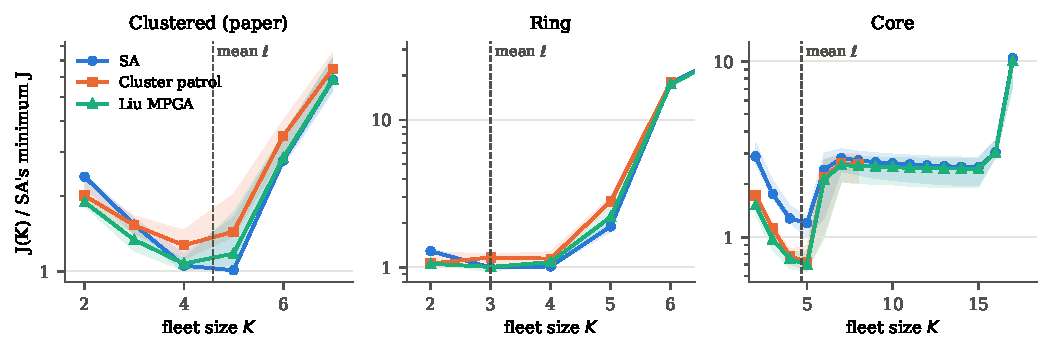
\includegraphics[width=\linewidth]{fig_fifty.pdf}
\caption{$J(K)$ divided by SA's per-instance minimum (log scale). Lines are the median over 12 seeds and
bands the interquartile range. Each planner is drawn on the $K$ range it was run on. Dashed line: mean
point predictor $\ell$.}
\label{fig:fifty}
\end{figure}

\begin{table}[H]\centering\small
\begin{tabularx}{\linewidth}{lL}
\toprule
Layout & median $J_{\mathrm{Liu}}/J_{\mathrm{SA}}$ per $K$ ($M=50$)\\
\midrule
\inputtab{perk_fifty.tex}
\bottomrule
\end{tabularx}
\caption{Paired per-$K$ ratio of adapted Liu to SA (median over seeds), $K\le10$. For $K>10$ every
median lies in [\fiftyTailLo, \fiftyTailHi].}
\label{tab:perk}
\end{table}

\paragraph{Fleet size: the predictor holds under all three planners.}
The adapted Liu planner's optimal fleet size is within one UAV of the point predictor $\ell$ in
\fiftyLiuWOneRuleAll{} instances (paper \fiftypaperLiuWOneRule, ring \fiftyringLiuWOneRule, core
\fiftycoreLiuWOneRule), and exactly at $\ell$ in \fiftypaperLiuExRule, \fiftyringLiuExRule{} and
\fiftycoreLiuExRule{} of instances respectively. Cluster patrol also stays within one UAV in every
instance. No planner's optimum is censored. On the core layout, both fixed-territory planners sit
\emph{closer} to $\ell$ than SA does: SA's optimum drifts up to a mean of \fiftycoreSaAm{} UAVs against a
mean of \fiftycoreLiuAm{} for Liu, and SA is within one UAV of $\ell$ in only \fiftycoreSaWOneRule{} of
core instances. This upward drift is the stranding regime that the fleet-sizing paper reports for the core
family (a far minimum reached by abandoning the peripheral outlier). It is a property of SA's curve on this
layout, not of the rule.

\paragraph{AoI level depends on the layout.}
\begin{itemize}
\item \emph{Clustered (paper):} SA is better. At each planner's own optimum, Liu's median $J$ is
  \fiftypaperLiuGap{} relative to SA, and Liu wins \fiftypaperLiuBetter{} instances. Cluster patrol is
  \fiftypaperClGap{}.
\item \emph{Ring:} essentially a tie (Liu \fiftyringLiuGap, wins \fiftyringLiuBetter).
\item \emph{Core:} the fixed-territory planners are far better. Liu is \fiftycoreLiuGap{} and cluster patrol
  \fiftycoreClGap{}, each winning \fiftycoreLiuBetter{} and \fiftycoreClBetter{} instances.
\end{itemize}
Per $K$ (Table~\ref{tab:perk}), Liu's advantage is concentrated at small fleets (median ratio
\fiftypaperLiuKtwo{} at $K=2$ on paper, \fiftyringLiuKtwo{} on ring, \fiftycoreLiuKtwo{} on core). On
paper and ring it disappears by $K\approx4$. On core it persists up to $K=5$ and then narrows as stranding
sets in for every planner.

\paragraph{Comparison with the original paper's own baseline findings.}
The fleet-sizing paper reports that the published cluster policy is about 32\% worse than SA on clustered
fields and about 31\% better on core. Here, at $M=50$, cluster patrol is \fiftypaperClGap{} on paper and
\fiftycoreClGap{} on core, so the direction and size match. The adapted Liu planner keeps the core
advantage of fixed territories, and on clustered fields it closes most of cluster patrol's gap to SA
(\fiftypaperLiuGap{} against \fiftypaperClGap). If an operator fixes the fleet at SA's predicted $\ell$,
Liu's $J$ relative to SA is \fiftypaperLiuAtRule{} (paper), \fiftyringLiuAtRule{} (ring) and
\fiftycoreLiuAtRule{} (core).

\paragraph{What this means for the fleet-sizing paper.}
The claim that the optimal fleet size is set by the rule and is stable across planners is
\textbf{supported}, now including a GA-optimised territorial planner from the literature on all three
layouts. A claim that SA gives the lowest AoI holds only on clustered fields at $M=50$. It does not hold on
core, where it was already known not to, or clearly on ring.

\subsection{Secondary check: $M=40$ (paper and ring)}
\begin{table}[H]\centering\small
\begin{tabular}{lrrrrrrrrr}
\toprule
 & & mean & \multicolumn{2}{c}{$\arg\min$ vs $\ell$} & $\arg\min$ & $J$ at own & wins & $J$ at & \\
Planner & $n$ & $\arg\min$ & exact & $\pm1$ & vs SA $\pm1$ & opt.\ vs SA & vs SA & $\ell$ vs SA & cens.\\
\inputtab{tab_forty.tex}
\bottomrule
\end{tabular}
\caption{The controlled $M=40$ set (paper and ring), same columns as Table~\ref{tab:fifty}.}
\end{table}

\noindent At $M=40$ the fleet-size result is the same: Liu's optimum is within one UAV of $\ell$ in
\fortyLiuWOneRuleAll{} instances. The AoI comparison is less favourable to SA. Liu's median $J$ at its
own optimum is \fortypaperLiuGap{} on paper (wins \fortypaperLiuBetter) and \fortyringLiuGap{} on ring
(wins \fortyringLiuBetter). On the clustered layout, then, the sign of the SA--Liu difference changes
between $M=40$ (Liu ahead) and $M=50$ (SA ahead). With 12 seeds per cell and differences of a few
percent, the AoI ordering of SA and Liu on clustered fields should be reported as \emph{comparable}, not
as a win for either planner.

%=====================================================================================================
\section{Caveats}
\begin{itemize}
\item \textbf{This is an adaptation, not the authors' code.} Every change is listed in Section~2. The two
  that matter most are the fitness (our surrogate) and nonstop deployment (sortie cutting).
\item \textbf{Strong by construction.} The baseline is Liu's search method optimising our objective. In
  structure it is a GA-searched fixed-territory patrol, of the same kind as the C4 scheduler of the
  fleet-sizing paper. It should not be presented as a weak baseline.
\item \textbf{No live adaptation.} Territories and sequences are fixed at the first launch. Only the
  commitment exclusion and the hover-energy estimate react to live state.
\item \textbf{Fixed GA seed.} Each $(\text{instance},K)$ uses RNG seed 0. Sensitivity to the seed was not
  measured.
\item \textbf{Different $M$ across studies.} The three-layout study uses $M=50$, because stored SA results
  for core exist only at $M\in\{50,100,200\}$. The $M=40$ set covers paper and ring only.
\end{itemize}

\section{Reproduction}
\begin{verbatim}
python baselines/liu2022/test_liu.py
python baselines/liu2022/run_m40.py baselines/liu2022/results/m40_liu.csv
python baselines/liu2022/run_m40.py baselines/liu2022/results/m50_liu.csv \
       --ref data/sa_rerun.csv --M 50 --Emax 1.5e6
python baselines/liu2022/report/make_report.py
tectonic baselines/liu2022/report/report.tex
\end{verbatim}

\end{document}
